\begin{equation}
\begin{gathered}
    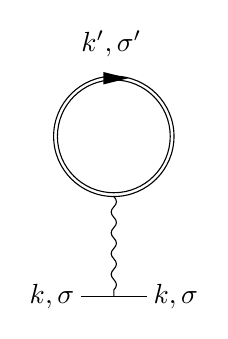
\begin{tikzpicture}[x=0.75pt,y=0.75pt,yscale=-1,xscale=1]
        %uncomment if require: \path (0,300); %set diagram left start at 0, and has height of 300
        
        %Shape: Circle [id:dp9029036047575749] 
        \draw   (142.85,180.48) .. controls (142.85,164.46) and (155.84,151.48) .. (171.85,151.48) .. controls (187.87,151.48) and (200.85,164.46) .. (200.85,180.48) .. controls (200.85,196.5) and (187.87,209.48) .. (171.85,209.48) .. controls (155.84,209.48) and (142.85,196.5) .. (142.85,180.48) -- cycle ;
        %Straight Lines [id:da07009274753482031] 
        \draw    (178.85,152.48) ;
        \draw [shift={(178.85,152.48)}, rotate = 180] [fill={rgb, 255:red, 0; green, 0; blue, 0 }  ][line width=0.08]  [draw opacity=0] (12,-3) -- (0,0) -- (12,3) -- cycle    ;
        %Shape: Circle [id:dp14502415990340833] 
        \draw   (144.68,180.48) .. controls (144.68,165.47) and (156.84,153.3) .. (171.85,153.3) .. controls (186.86,153.3) and (199.03,165.47) .. (199.03,180.48) .. controls (199.03,195.49) and (186.86,207.66) .. (171.85,207.66) .. controls (156.84,207.66) and (144.68,195.49) .. (144.68,180.48) -- cycle ;
        %Straight Lines [id:da5317389954978895] 
        \draw    (171.85,209.48) .. controls (173.52,211.15) and (173.52,212.81) .. (171.85,214.48) .. controls (170.18,216.15) and (170.18,217.81) .. (171.85,219.48) .. controls (173.52,221.15) and (173.52,222.81) .. (171.85,224.48) .. controls (170.18,226.15) and (170.18,227.81) .. (171.85,229.48) .. controls (173.52,231.15) and (173.52,232.81) .. (171.85,234.48) .. controls (170.18,236.15) and (170.18,237.81) .. (171.85,239.48) .. controls (173.52,241.15) and (173.52,242.81) .. (171.85,244.48) .. controls (170.18,246.15) and (170.18,247.81) .. (171.85,249.48) .. controls (173.52,251.15) and (173.52,252.81) .. (171.85,254.48) -- (171.85,257.5) -- (171.85,257.5) ;
        %Straight Lines [id:da07987340578000723] 
        \draw    (156,257.5) -- (187.71,257.5) ;
        
        % Text Node
        \draw (154,257.5) node [anchor=east] [inner sep=0.75pt]    {$\boldsymbol{k} , \sigma $};
        % Text Node
        \draw (155,128.4) node [anchor=north west][inner sep=0.75pt]    {$\boldsymbol{k}' , \sigma'$};
        % Text Node
        \draw (189.71,257.5) node [anchor=west] [inner sep=0.75pt]    {$\boldsymbol{k} , \sigma$};
        \end{tikzpicture}                 
\end{gathered} = \sum_{\vb*{k}', \sigma'} \expval*{n_{\vb*{k}' \sigma'}} \eval{\frac{- \ii 4 \pi e^2}{\abs*{\vb*{q}}^2}}_{\vb*{q} \to 0},
\end{equation}